\section{Simulation}
\label{sec:simulation}

\par In this section, we used NGspice in order to simulate the conceived AC/DC converter. In order to simplify the circuit, we had to make some changes.
\par Firstly, the transformer was replaced by an ideal model that consists in a pair of dependent sources (a current one in the primary circuit, and a voltage one in the secondary circuit). It should be noted that the values of the parameter n (parameter of dependency of the dependent sources), the capacitance of the capacitor and the resistance of the resistors were being adjusted through trial and error, in order to get an output voltage that is as close to 12V and as stable as possible.
\par In the tables below, the values of the ripple and the mean value of the voltage output for the envelope detector and the voltage regulator are shown.

\vspace{5mm}
\begin{table}[h!]
\centering
\begin{tabularx}{0.6\textwidth} {
  | >{\raggedright\arraybackslash}X
  | >{\raggedleft\arraybackslash}X | }
 \hline
@ca[i] & 0.000000e+00\\ \hline
@gb[i] & -2.68449e-04\\ \hline
@r1[i] & 2.563813e-04\\ \hline
@r2[i] & -2.68449e-04\\ \hline
@r3[i] & -1.20678e-05\\ \hline
@r4[i] & 1.186012e-03\\ \hline
@r5[i] & -2.68449e-04\\ \hline
@r6[i] & 9.296302e-04\\ \hline
@r7[i] & 9.296302e-04\\ \hline
v(1) & 5.125559e+00\\ \hline
v(2) & 4.861047e+00\\ \hline
v(3) & 4.313554e+00\\ \hline
v(5) & 4.898549e+00\\ \hline
v(6) & 5.710299e+00\\ \hline
v(7) & -1.91255e+00\\ \hline
v(8) & -2.87912e+00\\ \hline
v(9) & -1.91255e+00\\ \hline

\end{tabularx}
\caption{\label{tab:Table 3} Ripple and mean value for the envelope detector (all values are in Volt)}
\end{table}
\vspace{5mm}

\begin{table}[h!]
\centering
\begin{tabularx}{0.6\textwidth} {
  | >{\raggedright\arraybackslash}X
  | >{\raggedleft\arraybackslash}X | }
 \hline
@gb[i] & -1.07836e-18\\ \hline
@r1[i] & 1.029487e-18\\ \hline
@r2[i] & -1.07836e-18\\ \hline
@r3[i] & -4.88721e-20\\ \hline
@r4[i] & -2.21871e-19\\ \hline
@r5[i] & -1.89416e-03\\ \hline
@r6[i] & -2.16840e-19\\ \hline
@r7[i] & -4.26567e-19\\ \hline
v(1) & 0.000000e+00\\ \hline
v(2) & -1.03645e-15\\ \hline
v(3) & -3.22879e-15\\ \hline
v(5) & -8.88178e-16\\ \hline
v(6) & 5.930624e+00\\ \hline
v(7) & 4.540420e-16\\ \hline
v(8) & 8.881784e-16\\ \hline
v(9) & 4.540420e-16\\ \hline

\end{tabularx}
\caption{\label{tab:Table 4} Ripple and mean value for the voltage regulator (all values are in Volt)}
\end{table}
\vspace{5mm}

\par The following pictures show the plots for the input of the secondary circuit of the transformer (v(2)), the output voltage of the envelope detector (v(4)), the output voltage of the voltage regulator (v(5)), and the value of v(5)-12 (in order to show that it is a line close to zero - not completely straight because of the diodes, that are not linear components). Here we can see that the envelope detector does, in fact, decrease the ripple value, and the voltage regulator keeps the output voltage approximately constant.


\begin{figure}[h!] \centering
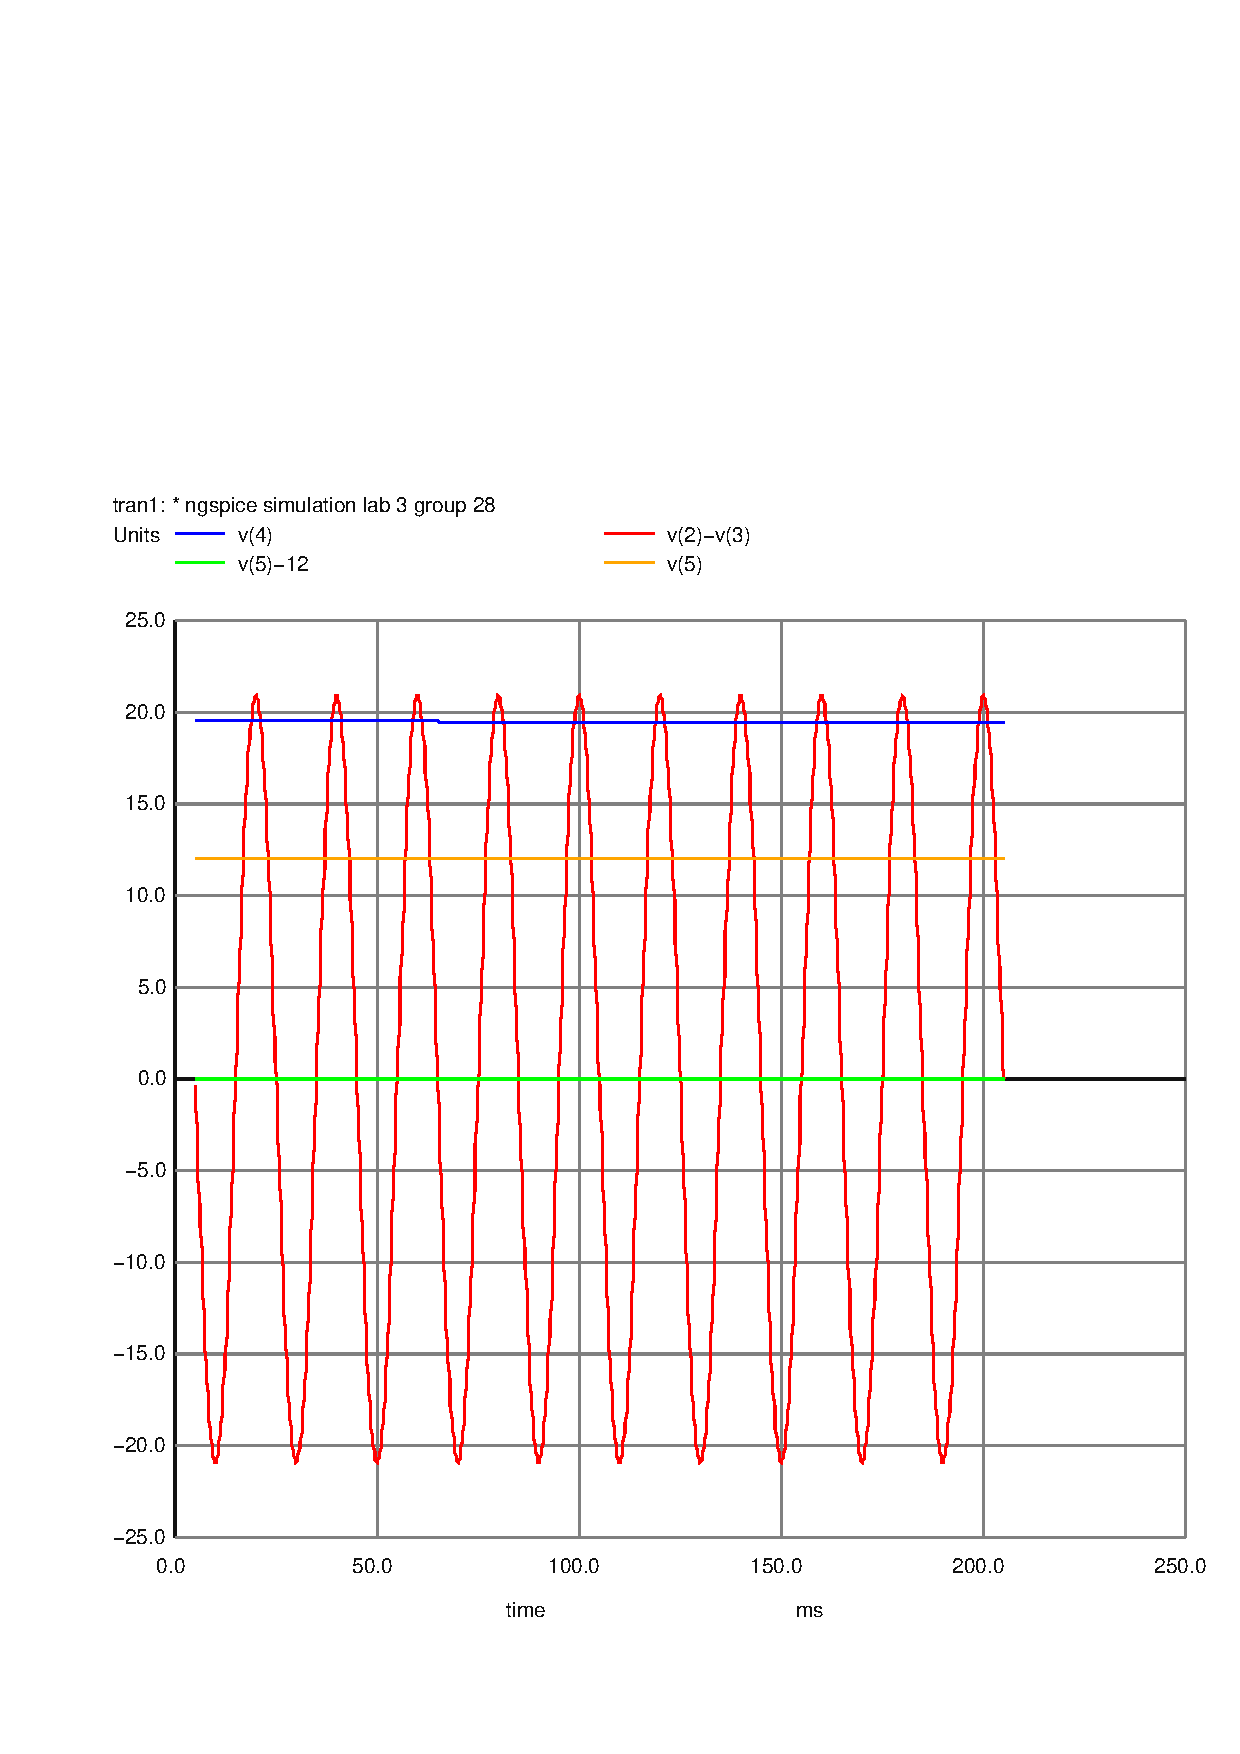
\includegraphics[width=0.6\linewidth]{sim3.pdf}
\caption{Input voltage of the secondary circuit (v(2)), output voltages of the envelope detector (v(4)) and voltage regulator (v(5)), and v(5)-12}
\end{figure}

\begin{figure}[h!] \centering
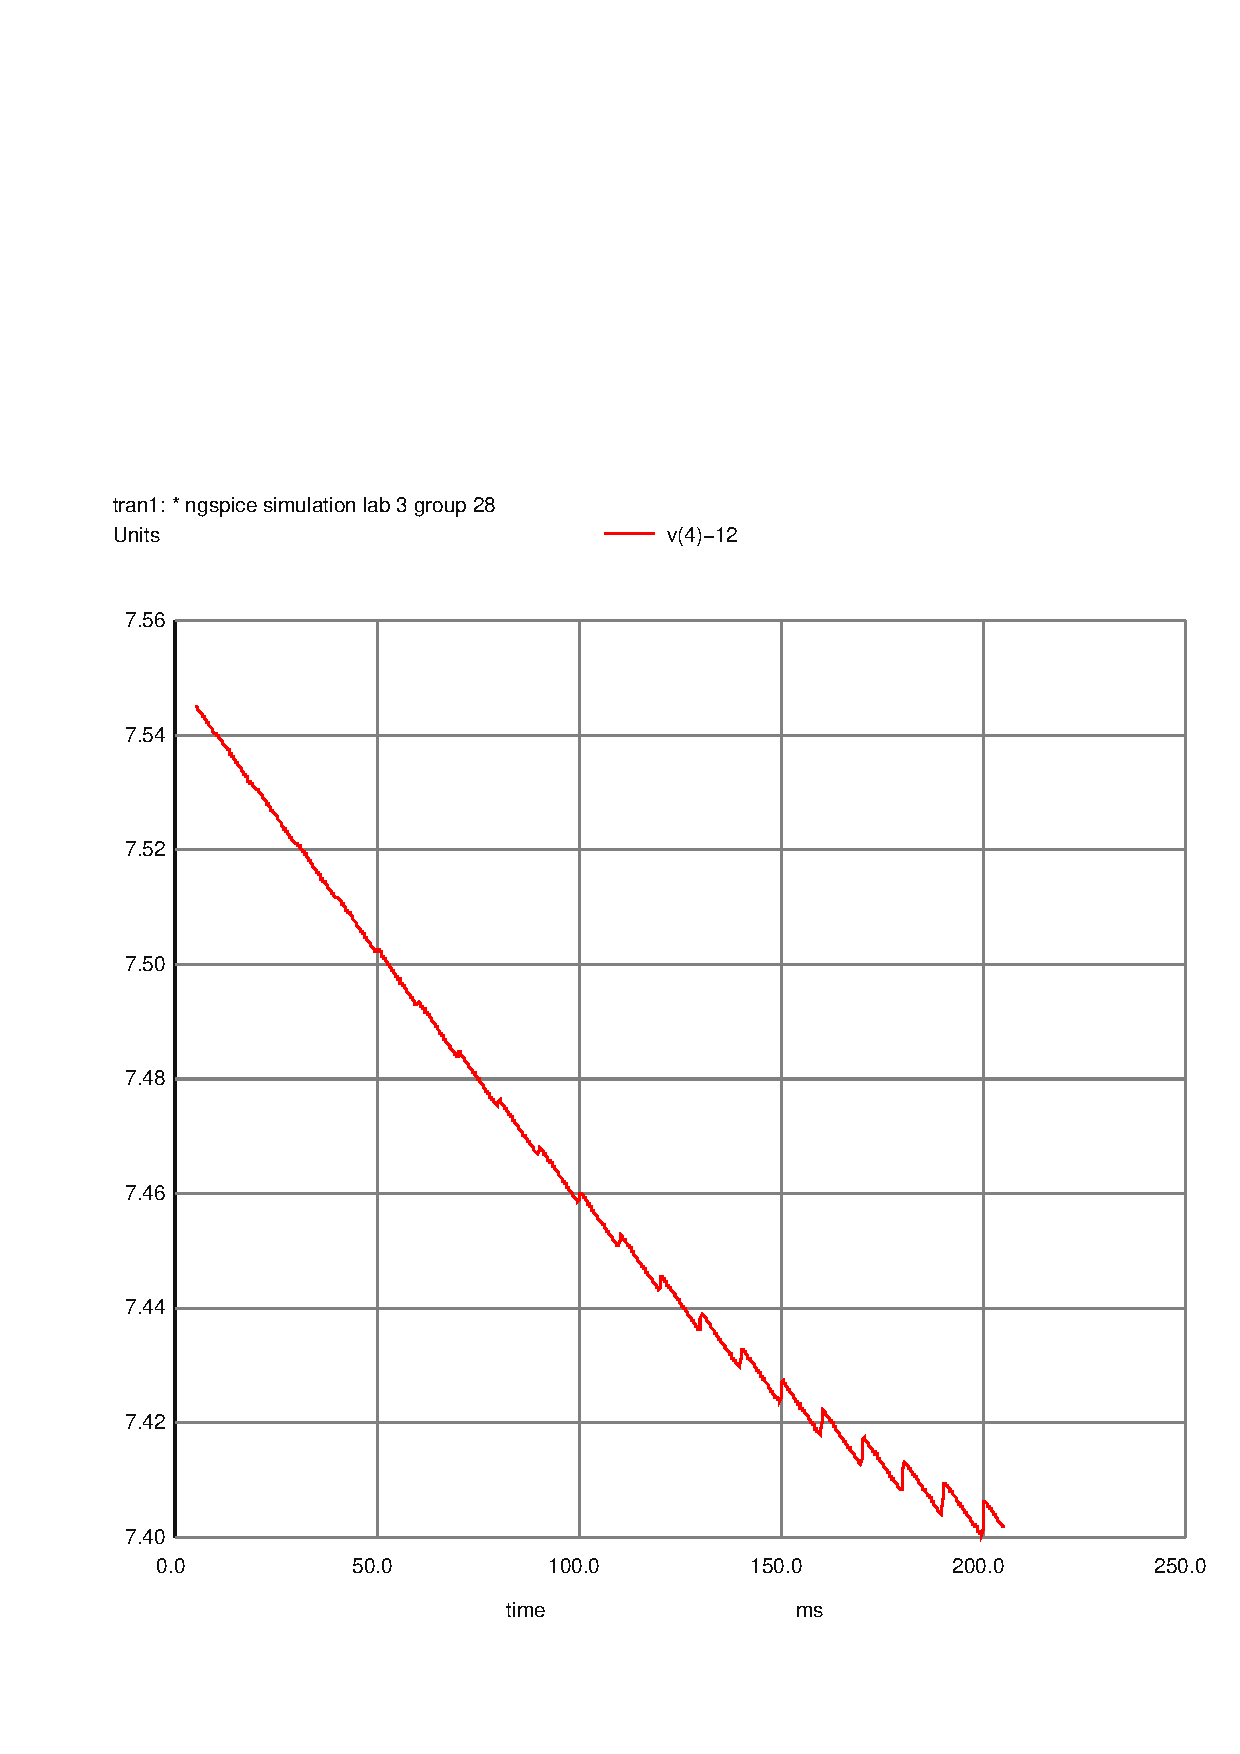
\includegraphics[width=0.6\linewidth]{sim31.pdf}
\caption{Total output deviation}
\end{figure}
